\documentclass{beamer}
% 
% Choose how your presentation looks.
% 
% For more themes, color themes and font themes, see:
% http://deic.uab.es/~iblanes/beamer_gallery/index_by_theme.html
% 
\mode<presentation>
{
  \usetheme{default}      % or try Darmstadt, Madrid, Warsaw, ...
  \usecolortheme{beaver} % or try albatross, beaver, crane, ...
  \usefonttheme{default}  % or try serif, structurebold, ...
  \setbeamertemplate{navigation symbols}{}
  \setbeamertemplate{caption}[numbered]
} 

\usepackage{graphicx}
\usepackage[english]{babel}
\usepackage[utf8x]{inputenc}
\usepackage{url}

\newcommand\heading[1]{%
  \par\bigskip
  {\Large\bfseries#1}\par\smallskip}

\title[Version Control Intro]{Version Control: What and Why}
\author{Andy Choens, MSW}
\institute{Office of Quality and Patient Safety}
\date{May 20, 2015}

\begin{document}

\begin{frame} %-----------------------------------------------------------------
  \titlepage
\end{frame}

\begin{frame}{Outline} % -------------------------------------------------------
  \tableofcontents
\end{frame}

\section{Introduction} %% ======================================================

\begin{frame} % ----------------------------------------------------------------
  \frametitle{Dafynitions}
  \begin{itemize}
  \item \textbf{Version Control:} \textit{the management of changes to documents,
    computer programs, large web sites, and other collections of
    information.\footnote{https://en.wikipedia.org/wiki/Revision\_control}
    It has many names.
    \begin{itemize}
    \item Revision Control
    \item Source Control
    \item Renaming Files
    \item VC
    \end{itemize}}
  \item \textbf{Git:} \textit{a distributed revision control system with an
    emphasis on speed, data integrity, and support for distributed,
    non-linear
    workflows. \footnote{https://en.wikipedia.org/wiki/Git\_(software)}}
  \item \textbf{GitLab:} \textit{a web-based Git repository manager with wiki
    and issue tracking features. GitLab is similar to GitHub, but
    GitLab has an open source version, unlike
    GitHub.\footnote{https://en.wikipedia.org/wiki/GitLab}}
  \end{itemize}
\end{frame}  

\begin{frame} % ----------------------------------------------------------------
  \frametitle{Git and R:}  
  \begin{itemize}
  \item VC and git are heavily used by the R community.
  \item You can use git for SAS development as easily as R.
  \item Or Excel . . . . 
  \item Or a Presentation . . . .
  \end{itemize}
\end{frame}

\begin{frame} % ----------------------------------------------------------------
  \frametitle{After The Show:}

  \textbf{Today:}
  \begin{itemize}
  \item What and Why.
  \item Not How.
  \item Git isn't rocket science. . . or epidemiology.
  \end{itemize}

  \bigskip
  \textbf{On Your Own:}
  \begin{itemize}
  \item {\url{https://msysgit.github.io/}}
  \item {\url{http://sourceforge.net/projects/gitextensions/}} BLOCKED!
  \item {\url{http://doc.gitlab.com/ce/}}
  \item {\url{https://help.github.com/}}
  \end{itemize}

  \bigskip
  \textbf{This presentation can be found at:}
  \begin{itemize}
  \item {\small{\url{https://github.com/choens/git-for-research-scientists}}}
  \end{itemize}
  
\end{frame}

\begin{frame} % ----------------------------------------------------------------
  \frametitle{When Version Control Matters}
  
  \begin{columns}
    \begin{column}{.5\textwidth}
      \begin{itemize}
      \item \textbf{Q:} \textit{Is all this relevant to me?}
      \item \textbf{A:} \textit{Yes.}
      \end{itemize} 
    \end{column}
    
    \begin{column}{.5\textwidth}
        \centering
        
\includegraphics[height=.8\textheight]{img/final} 
    \end{column}
  \end{columns}
  \footnote{http://www.phdcomics.com/comics/archive.php?comicid=1531}
\end{frame}

\section{Informal Version Control} %% ==========================================

\begin{frame} % ----------------------------------------------------------------
  \frametitle{Informal Version Control: Examples}
  {\large Woefully incomplete list of examples:}
  \bigskip
  \begin{itemize}
  \item File-name spaghetti.
  \item Track Changes In Word, Excel, etc.
  \item DropBox, SpiderOak
  \item Time Machine in OSX
  \item Who else has a different USB drive for every day of the week?
  \end{itemize} 
\end{frame}

\begin{frame} % ----------------------------------------------------------------
  \frametitle{Informal Version Control: Examples 2}
  \begin{columns}[t]
    \begin{column}{.5\textwidth}
      \textbf{{\large Advantages}}
      \begin{itemize}
      \item Sometimes, it is built in.
        \begin{itemize}
        \item Word
        \item SAS
        \end{itemize}
      \item Easily implemented.
      \item You already know how.
      \end{itemize}
    \end{column}
    
    \begin{column}{.5\textwidth}
      \textbf{{\large Disadvantages}}
      \begin{itemize}
      \item Not equally available.
        \begin{itemize}
        \item PowerPoint
        \item Data revisions?
        \end{itemize}
      \item Only starts simple.
      \item I hope everyone agrees how.
      \item Multiple collaborators?
        \begin{itemize}
        \item Who changed the code?
        \item When?  
        \item Why?
        \item Which version do I have?
        \item Where is last year's code?
        \item What is branching?
        \end{itemize}
      \end{itemize}
    \end{column}
  \end{columns}
\end{frame}

\begin{frame} % ----------------------------------------------------------------
  \frametitle{Informal Version Control: Fail} 

  \textbf{Q:} Which SAS file generated the graph given to the
  Medicaid Director last fall?

  \bigskip
  \begin{itemize}
  \item big\_project/2014.05.27.run.sas
  \item big\_project/2014.05.27.re\_run.sas
  \item big\_project/2014.05.27.re\_re\_run.sas
  \item big\_project/2014.05.28.use\_this\_one.sas
  \item big\_project/2014.05.29.huh.sas
  \item big\_project/2014.05.30.aaaargh.sas
  \item big\_project/2014.05.31.not\_bad.sas
  \item big\_project/2014.05.31.woohoo.sas
  \end{itemize}

  \bigskip
  \begin{center}
  \textbf{Welcome To Informal Version Control.}
  \end{center}
  
\end{frame}

\begin{frame}  % ---------------------------------------------------------------
  \frametitle{Informal Version Control: FAILS}
  {\large Have you or a colleague ever . . . . }
  \bigskip
  \begin{itemize}
  \item Wasted all morning waiting for the shared drive to come back
    on-line?
  \item Been unable to reproduce the \emph{really} important graph
    given to the Medicaid Director last fall, because the code has
    been lost (overwritten)?
  \item Struggled to maintain two parallel code bases?
  \item Been unsure if the code you are using is the most current
    version? If it isn't, what are the changes and where are they in
    the code?
  \end{itemize}
\end{frame}


\section{Formal Version Control} %% ============================================

\begin{frame} % ----------------------------------------------------------------
  \frametitle{Formal Version Control: The Answer}

  \textbf{Gives users tools, practices and community norms that enable
    more effective collaboration and communication.}
  
 \end{frame}
 
\begin{frame} % ----------------------------------------------------------------
  \frametitle{Formal Version Control: Wikipedia Example}
  
  \begin{itemize}
  \item Version Control can be found in lots of places, like
    Wikipedia\footnote{\url{https://en.wikipedia.org/wiki/Help:Page_history}}.
  \item The entire history of EVERY Wikipedia Article is available.
  \item Wikipedians place a high priority in understanding how their
    product changes over time.
  \item They have a common system for sharing, tracking and using
  changes to their product.
  \item There is not reason we can't have the same history for the
    work we do.
  \end{itemize}

\end{frame}

\begin{frame}  % ---------------------------------------------------------------
  \frametitle{Formal Version Control: WINS}
  {\large Have you or a colleague ever:}
  \bigskip
  \begin{itemize}
  \item Wasted all morning waiting for the shared drive to come back
    on-line?
  \item Been unable to reproduce the \emph{really} important graph
    given to the Medicaid Director last fall, because the code has
    been lost (overwritten)?
  \item Struggled to maintain two parallel code bases?
  \item Been unsure if the code you are using is the most current
    version? If it isn't, what are the changes and where are they?
  \end{itemize}

  \begin{center}
    \textbf{Let's turn these FAILS into WINS!}
  \end{center}
\end{frame}

\begin{frame} % ----------------------------------------------------------------
  \frametitle{Have you or a colleague ever . . . . \# 1} 
 
  \textbf{Fail:} Wasted all morning waiting for the shared drive to
  come back on-line?
 
  \medskip 
  \noindent\makebox[\linewidth]{\rule{\textwidth}{0.4pt}}
  \medskip

  \textbf{Win:} Git stores a local copy of the code on YOUR local
  computer. If the server goes down, you can still work, but you can't
  collaborate.
  
\end{frame}
 
\begin{frame} % ----------------------------------------------------------------
  \frametitle{Have you or a colleague ever . . . . \# 2} 

  \textbf{Fail:} Been unable to reproduce the \emph{really} important
  graph given to the Medicaid Director last fall, because the code has
  been lost (overwritten)?

  \medskip 
  \noindent\makebox[\linewidth]{\rule{\textwidth}{0.4pt}}
  \medskip

  \textbf{Win:} Committed changes are a permanent part of the project\footnote{\url{http://appdev1/oqps/hh-quarterly-qa-report/commits/master}}.
  
  \medskip
  \textbf{Win:} Code state at commit is always reproducible.

  \medskip
  \textbf{Win:} Important versions can be tagged\footnote{\url{http://appdev1/oqps/hh-quarterly-qa-report/tags}}.
  
\end{frame}

\begin{frame}
  \frametitle{This Is A Practice, Not A Guarantee}
  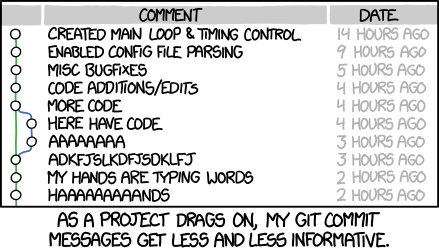
\includegraphics[width=\textwidth]{./img/git_commit.png}\footnote{\url{https://xkcd.com/1296/}}
\end{frame}
 
\begin{frame} % ----------------------------------------------------------------
  \frametitle{Have you or a colleague ever . . . . \# 3}

  \textbf{Fail:} Struggled to maintain two parallel code bases? (Vertica?)

  \medskip 
  \noindent\makebox[\linewidth]{\rule{\textwidth}{0.4pt}}
  \medskip

  \textbf{Win:} Branches: You can maintain many parallel code
  bases easily\footnote{\url{http://appdev1/axc38/hp-cmart/network/master}}.

\end{frame}
 
\begin{frame} % ----------------------------------------------------------------
  \frametitle{Have you or a colleague ever . . . . \# 4} 

  \textbf{Fail:} Been unsure if the code you are using is the most
  current version? If it isn't, what are the changes and where are they?
  
  \medskip 
  \noindent\makebox[\linewidth]{\rule{\textwidth}{0.4pt}}
  \medskip

  \textbf{Win:} Git repos  contain the full history \& status of a project\footnote{\url{http://appdev1/oqps/hh-quarterly-qa-report/merge_requests}}.

  \medskip
  \textbf{Win:} Tools to sync the local copy to the remote
  master. (git pull)

\end{frame}

\begin{frame} % ----------------------------------------------------------------
  \frametitle{Git + Gitlab == Project Management}
  \begin{itemize}
  \item Central place to share scientific code and projects
  \item  1 repo == 1 project
  \item Tracks changes in files over time\footnote{\url{http://appdev1/oqps/hh-quarterly-qa-report/commits/master}}
  \item Issues / Bug Tracking\footnote{\url{http://appdev1/oqps/hh-quarterly-qa-report/issues}}
  \item Tools for
    collaboration
    \footnote{\url{http://appdev1/care-management/hp-cmart-reports/issues/1}}
  \end{itemize}
\end{frame}

\begin{frame} % ----------------------------------------------------------------
  \frametitle{What Happens Next?}
  \begin{itemize}
  \item This is a different way of working, but anyone can learn it.
  \item I am developing some formal training materials with EBCOP.
  \item Don't forget the links from the beginning of the presentation.
  \item File an ITS ticket to get MSYS Git and Git Extensions.
  \item For GitLab: Contact Jeremy Redmond and Avideh Sadaghiani.
  \item Questions? Post it to the EBCOP blog and we can discuss.
  \end{itemize}
\end{frame}

\section{Questions?} %% ========================================================

\begin{frame} % ----------------------------------------------------------------
 \frametitle{Questions?}
 
\includegraphics[width=\textwidth]{./img/questions.png}
\end{frame}

\end{document}
